

\usepackage{tikz}
\usepackage[utf8]{inputenc}
\usepackage{amsmath}
\usepackage{amsfonts}
\usepackage{amssymb}
\usepackage{stackrel}
%\usepackage{kpfonts}
\usepackage{amssymb, amsmath, amsbsy} 
\usepackage{makeidx}
\usepackage{graphicx}
\usepackage{multicol}
\usepackage{changepage}
\usepackage{float}
\usepackage{cite}
\usepackage{pstricks, caption}
\usepackage{url}
\usepackage[spanish, es-tabla]{babel}
\usepackage[shortlabels]{enumitem}
\usepackage{longtable,multirow,booktabs}
\usepackage{rotating}
\usepackage{caption}
\usepackage{multirow, array}
\usepackage{anyfontsize}
\usepackage{fix-cm}
\usepackage{calligra}
\usepackage{mathptmx}
\usepackage{caption}
\usepackage{fancyvrb}
%\usepackage{esvect}
\usepackage{xargs}
\usepackage{subfigure} 
\usepackage {titletoc}
\usepackage[T1]{fontenc}

\documentclass[13,twocolumn,letterpaper]{article}
    \usepackage[spanish,english]{babel}
    \usepackage[utf8x]{inputenc}
    \usepackage[T1]{fontenc}
    \usepackage[a4paper,top=3cm,bottom=2cm,left=3cm,right=3cm,marginparwidth=1.75cm]{geometry}
    \usepackage{amsmath}
    \usepackage[colorinlistoftodos]{todonotes}
    \usepackage[colorlinks=true, allcolors=blue]{hyperref}
    \usepackage{float}
    
    
 \spanishdecimal{.}
\renewcommand{\figurename}{\textbf{Figura}}
\renewcommand{\tablename}{\textbf{Tabla}}
\renewcommand{\refname}{Bibliografía}
\renewcommand{\abstractname}{\large\textbf{Resumen}}
\renewcommand{\contentsname}{Contenido}
\renewcommand{\partname}{Parte}
\renewcommand{\appendixname}{Apéndice}
\renewcommand{\sin}{sen}	
\newenvironment{Figure}{\par\medskip\noindent\minipage{\linewidth}}{\endminipage\par\medskip}

    
    \title{
    		%\vspace{-1in} 	
    		\usefont{OT1}{bch}{b}{n}
    		\normalfont \normalsize \textsc{INSTITUTO POLITÉCNICO NACIONAL \\ 
    		ESCUELA SUPERIOR DE FISICA Y MATEMATICAS \\
    		ACADEMIA DE FÍSICA EXPERIMENTAL} \\ [10pt]
    		\huge Práctica V:\\
    Determinaci\'on de Longitud Focal de Espejos Esféricos.\\
    }
    
    \usepackage{authblk}
    \author[0]{Alumno: Flores Rodriguez Jaziel David \\
    Boleta: 2014030429 \\
    Profesor: Dr. Janos Zsargo\\
    Grupo: 4FV2-B \\
            }
\begin{document}

\maketitle
 \section*{Resumen}
El objetivo principal fue el de determinar mediante diversos experimentos la distancia focal de espejos esféricos. Para lograr esto la actividad experimental se dividi\'o en tres partes, en la primera de ellas se determinó la distancia focal de manera directa, en la segunda parte medimos el radio de curvatura con un esferómetro, a partir del radio se determino la distancia focal.  Y la ultima parte experimental se determino la distancia focal mediante el método de autocolimación

\\
\section*{Introducción }
{ 
Los espejos curvos se clasifican convenientemente como esféricos y no esféricos. En la figura 1 se muestran algunas configuraciones no esféricas.

\begin{figure}[h!]
	\centering
	\subfigure{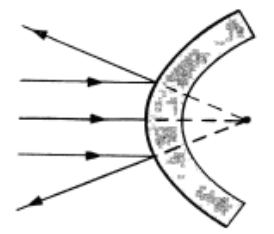
\includegraphics[scale=0.29]{fig1a}}
	\hspace{1 cm}
	\subfigure{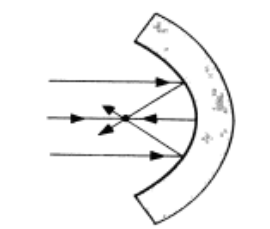
\includegraphics[scale=0.29]{fig1b}}
	\hspace{1 cm}
	\subfigure{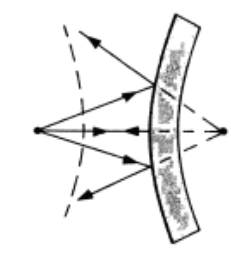
\includegraphics[scale=0.26]{fig1c}}\\
	\subfigure{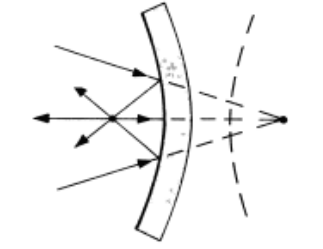
\includegraphics[scale=0.281]{fig1d}}
	\hspace{0.5 cm}
	\subfigure{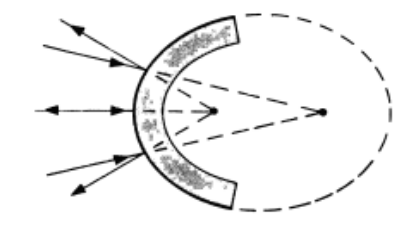
\includegraphics[scale=0.29]{fig1e}}
	\hspace{0.5 cm}
	\subfigure{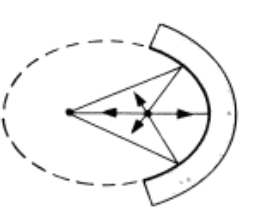
\includegraphics[scale=0.35]{fig1f}}
	\caption{{\small  {(a) Parabólico convexo. (b) Parabólico cóncavo. (c) Hiperbólico convexo. (d) Hiperbólico cóncavo (e) Elíptico convexo. (f) Elíptico cóncavo.}}}
	\label{fig:fig1}
\end{figure}


	La ecuación paraxial que relaciona el objeto conjugado y puntos imagen con los parámetros físicos de un espejo esférico pueden deducirse de manera muy simple con la ayuda de la figura 2. Para ello notemos que  $\theta_{i}=\theta_{r}$ el $\measuredangle SAP$ es cortado en dos partes iguales por $\overline{CA}$, que por consiguiente divide al lado $\overline{SP}$ del triangulo $SAP$ en segmentos proporcionales a los dos lados restantes, esto es
\begin{equation}
\dfrac{\overline{SC}}{\overline{SA}}=\dfrac{\overline{CP}}{\overline{PA}}
\end{equation}
	Además
	$$\overline{SC}=s_{0}-|R|$$
	y
	$$\overline{CP}=|R|-s_{i}$$
	donde $s_{0}$ y $s_{i}$ están a la izquierda siendo, por lo tanto, positivas. Si utilizamos la misma convención de signos que la usada comúnmente en temas de refracción, $R$ será negativa por que $C$ se halla  a la izquierda de $V$ es decir, la superficie es cóncava. 
	 
\begin{figure}
\begin{minipage}[b]{0.42\textwidth}
	\begin{center}
		\subfigure{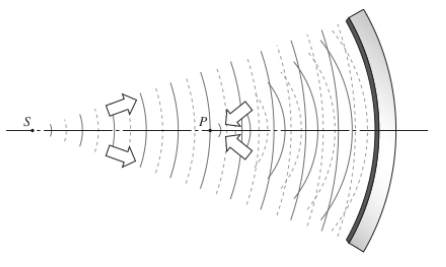
\includegraphics[scale=0.6]{fig2a}}\\
		\subfigure{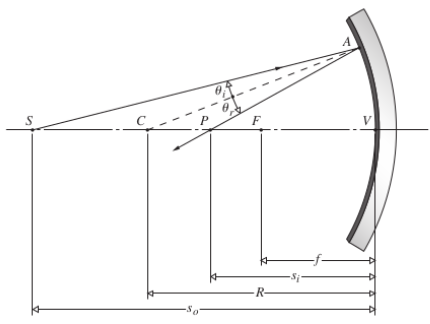
\includegraphics[scale=0.6]{fig2b}}
		\caption{Espejo esférico cóncavo. Focos conjugados }
	\end{center}
\end{minipage}
\end{figure}

Entonces $|R|=-R$ y 
$$\overline{SC}=s_0+R$$
y $$\overline{CP}=-(s_{0}+R)$$
En la región paraxial $\overline{SA}\approx s_{0}$, y $\overline{PA}\approx s_{i}$, así la ecuación (1) queda
$$\dfrac{s_{0}+R}{s_{0}}=-\dfrac{s_{i}+R}{s_{i}}$$
o bien 
\begin{equation}
\dfrac{1}{s_{0}}+\dfrac{1}{s_{i}}=-\dfrac{2}{R}
\end{equation}
La ecuación (2) se denomina la \textbf{fórmula de los espejos}. Es aplicable tanto a espejos cóncavos $(R<0)$ como convexos $(R>0)$. El \emph{foco objeto } o \emph{primario} se define por 
$$\lim_{s_{i}\rightarrow\infty}s_{0}=f_{0}$$
mientras que el \emph{foco imagen} o \emph{secundario} corresponde a 
$$\lim_{s_{0}\rightarrow\infty}s_{i}=f_{i}$$
De la ecuación (2) se tiene que 
$$\dfrac{1}{f_{0}}+\dfrac{1}{\infty}=\dfrac{1}{\infty}+\dfrac{1}{f_{i}}=-\dfrac{2}{R}$$
Lo cual implica que
\begin{equation}
f_{0}=f_{i}=-\dfrac{R}{2}
\end{equation}
quitando los subíndices de las distancias focales se tiene que 
\begin{equation}
\dfrac{1}{s_{0}}+\dfrac{1}{s_{i}}=\dfrac{1}{f}
\end{equation}
}
\section*{Experimentos}
{
	La actividad experimental se dividió en tres experimentos, los cuales fueron el método directo, el método por la medición del radio de curvatura con un esferómetro y el método de autocolimación.
\subsection{Método directo}
{
El montaje experimental se puede observar en la figura 3
\begin{figure}[h!]
	\centering
	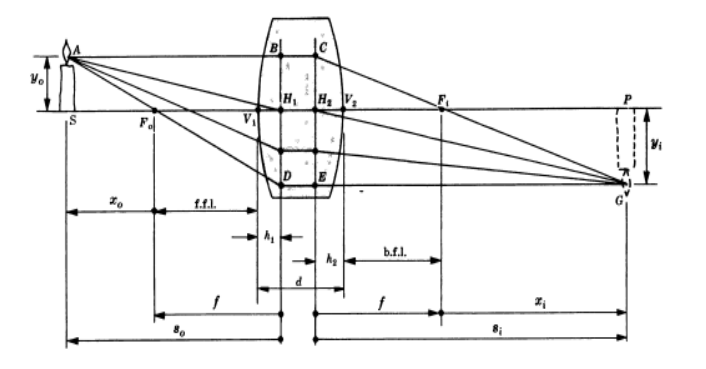
\includegraphics[width=0.8\linewidth]{fig3}
	\caption[fig 4]{Montaje experimental para el experimento del método directo.}
	\label{fig:fig3}
\end{figure}
\\Lo primero que se realizo fue incidir un haz de luz del láser sobre el espejo cóncavo, posteriormente sobre la pantalla se encontró el mejor punto de enfoque del haz reflejado por el espejo, y por ultimo se midió la distancia focal $f$, como se muestra en la figura 3, que no es nada más que la distancia de la pantalla al espejo.\\
Lo anterior lo realizamos con dos espejos.

}
\subsection*{Medición del radio de curvatura con un esferómetro}
{
	Para este experimento se determino el radio de curvatura de un ''espejo'' con un esferómetro, para ello se monto el experimento como se muestra en la figura 4, y se tomaron los datos que se muestran también en la figura 4, lo cuales fueron $h$ y $d$ para después usarlos en la siguiente ecuación
	\begin{equation}
	R=\dfrac{d^{2}}{6h}
	\end{equation}
	
	\begin{figure}[h!]
		\centering
		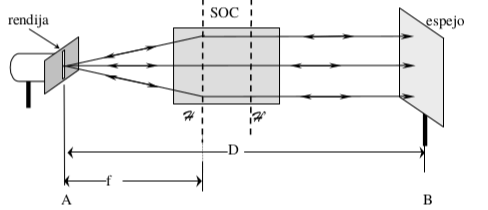
\includegraphics[width=0.7\linewidth]{fig4}
		\caption[fig 4]{Montaje experimental para la medición del radio de curvatura con un esferómetro.}
		\label{fig:fig4}
	\end{figure}
Además se tomo $h$ de dos formas distintas, con la profundidad $h$ tomada como se muestra en la figura 4 y con la profundidad $h$ tomada girando el espejo. 

}
\subsection*{Método de autocolimación}
{
	Se monto el experimento como se puede observar en la figura 5. Luego se realizo lo siguiente:\\ 
	Con la ayuda de una lente delgada primero encontramos la imagen real sobre la pantalla $B$, de la rendija ubicada en la pantalla $A$.\\
	Luego colocamos un espejo convexo entre la lente delgada y la pantalla $B$ (ver figura 5).\\
	Variamos la distancia del espejo a la pantalla $B$ hasta que se observo en la pantalla $A$ una imagen nítida de la rendija, en esta posición se asegura que $x_{1}-x_{2}=R$, donde $R$ es el radio de curvatura del espejo convexo.
	\\Se repitió lo anterior con otro espejo.
		\begin{figure}[h!]
		\centering
		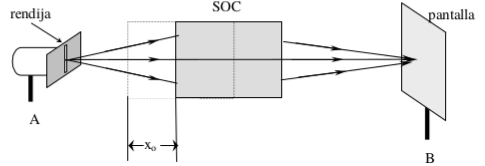
\includegraphics[width=0.7\linewidth]{fig5}
		\caption[fig 4]{Montaje experimental para el método de autocolimación.}
		\label{fig:fig5}
	\end{figure}
}

}


\section*{Datos obtenidos}
{

\subsection*{Método directo}
{
	Para este experimento se obtuvieron los siguientes datos:\\
	Para el primer espejo $(250\;mm)$:
	\begin{itemize}
		\item [ $1^{ra}$ ] $f_{1}=22.05\; cm$
		\item [ $2^{da}$ ] $f_{2}=21.95\; cm$
		\item [ $3^{ra}$ ] $f_{3}=23.25\; cm$
	\end{itemize}
El promedio de las mediaciones anteriores es de $\overline{f}=22.41\;cm$.
Para el segundo espejo $(120\;mm)$:
\begin{itemize}
	\item [ $1^{ra}$ ] $f_{1}=10.55\; cm$
	\item [ $2^{da}$ ] $f_{2}=10.75\; cm$
	\item [ $3^{ra}$ ] $f_{3}=11.25\; cm$
\end{itemize}
El promedio de las mediaciones anteriores es de $\overline{f}=10.85\;cm$.\\
}
\subsection{Medición del radio de curvatura con un esferómetro}
{
Para este experimento se obtuvieron los siguientes datos:\\
Con $h$ tomada como se indica la figura 4:
Para ambos casos $d=5.14 \;cm$ 
\begin{itemize}
	\item [ $1^{ra}$ ] $h=3.25\; mm $
	\item [ $2^{da}$ ] $h=3.22\; mm $
\end{itemize}
Su promedio fue $\overline{h}=3.235 \;mm$, utilizando la ecuación (5) se obtuvo el radio el cual es de $R=13.61 \;cm$, y $f=\dfrac{R}{2}=6.805\;cm$.\\
Con $h$ tomada al revés de  como se indica la figura 4:
\begin{itemize}
	\item [ $1^{ra}$ ] $h=3.23\; mm $
	\item [ $2^{da}$ ] $h=3.20\; mm $
\end{itemize}	
Su promedio fue $\overline{h}=3.215 \;mm$, utilizando la ecuación (5) se obtuvo el radio el cual es de $R=13.69 \;cm$  y $f=\dfrac{R}{2}=6.845\;cm$.
\\El radio del fabricante es de $R_{f}=13.16\;cm$ y  $f_{f}=6.58 \;cm$.
}
\subsection*{Método de autocolimación}
{
	
	
	Para este experimento se obtuvieron los siguientes datos:\\
	El espejo era de $250\;mm$, ademas $s_{0}=26.6 \;cm$ y $s_{i}=80.2 \;cm$, luego $$R=s_{i}-s_{0}=46.3\; cm$$
	y además $$f=\dfrac{R}{2}=23.15\;cm$$
	
}

}

\section*{Resultados}
{

\subsection*{Método directo}
{
Para el primer espejo se obtuvo el siguiente porcentaje de error:
$$\%e=\dfrac{|25.0\;cm - 22.41\;cm|}{25.0\; cm}\times 100=10.36\%$$
Para el segundo espejo
$$\%e=\dfrac{|12.0\;cm - 10.85\;cm|}{12.0\; cm}\times 100=9.58\%$$	
}
\subsection*{Medición del radio de curvatura con un esferómetro}
{
Con $h$ tomada como se indica la figura 4 su por ciento de error para el radio fue de:
$$\%e=\dfrac{|13.16\;cm - 13.61\;cm|}{13.16\; cm}\times 100=3.41\%$$
Y para $f$ el por ciento de error para el radio fue de:
$$\%e=\dfrac{|6.58\;cm - 6.805\;cm|}{6.58\; cm}\times 100=3.41\%$$
Con $h$ tomada al revés de  como se indica la figura 4 el porcentaje de error es de:	
$$\%e=\dfrac{|13.16\;cm - 13.69\;cm|}{13.16\; cm}\times 100=4.02\%$$
Y para $f$ el error porcentual para el radio fue de:
$$\%e=\dfrac{|6.58\;cm - 6.845\;cm|}{6.58\; cm}\times 100=4.02\%$$
}
\subsection*{Método de autocolimación}
{
El porcentaje de error para este método fue de
 	$$\%e=\dfrac{|25.0\;cm - 23.15\;cm|}{25.0\; cm}\times 100=7.4\%$$
}

}


\section*{Conclusiones}
{
El mecanismo óptico del los espejos es, en cierto modo diferente al de las lentes delgadas por lo que las ecuaciones de las lentes delgadas apenas y nos sirven para estudiar a los espejos esféricos, esto se puede observar en los resultados obtenidos en el método directo, pues de los tres métodos experimentales este fue en el que se obtuvo el mayor error porcentual, en cambio en el método de autocolimación el error bajo, claro que no como se esperaría, y en el método en el que se utilizo el esferómetro se obtuvieron los mejores resultados, pero hay que analizar más a fondo este resultado ya que no utilizamos un espejo como tal, si no mas bien utilizamos un lentes esférico dada la rareza (y la dificultad) que tendría conseguir un espejo esférico, aunque para nuestros fines los cuales no son más que estudiar los espejos esféricos en los tres métodos se obtuvieron, dentro de lo que se pide los resultados esperados.
\\ Incluso  dejando a un lado lo que se acaba de comentar, también hay que tener en cuenta la calidad de los materiales utilizados pues estos se han ocupado por varios compañeros a través del tiempo y esto implica un desgaste del material lo cual se ve reflejado en los resultados. 

}


\nocite{Hecht}\nocite{Rossi}\nocite{Sears}\nocite{Born}\nocite{Tipler}\nocite{Feynman}\nocite{Res}
\bibliography{miBiblio.bib}
\bibliographystyle{plain}
\end{document}